\chapter{DUNE Far Site Technical Coordination}
\label{ch:exec-tc}

%%%%%%%%%%%%%%%%%%%%%%%%%%%%%%%%%%%%%%%%%%%%%
\section{Overview}

Far site \dword{tc} concerns the organization and management of 
activities required to design, construct,
fabricate, install, and commission the \dword{dune} \dword{fd} modules properly and safely. 
      The \dword{dune} collaboration has direct responsibility for the design 
and construction of the \dword{dune} detectors.  Groups of collaborative 
institutes, referred to as consortia, assume responsibility for 
the different detector subsystems.  The activities of the consortia are 
overseen and coordinated through the \dword{dune} \dword{tc} organization 
headed by the \dword{dune} \dword{tcoord}.  The \dword{tc} organization 
provides project support functions such as safety coordination, 
engineering integration, change control, document management, scheduling, 
risk management, and technical review planning.  \dword{dune} \dword{tc} 
manages internal, subsystem-to-subsystem interfaces and ensures the proper integration of the different subsystems.   

\dword{dune} \dword{tc} works closely with the support teams of its 
\dword{lbnf-dune} partners within the framework of the \dword{jpo} to 
ensure project support functions across the entire global 
enterprise are coherent.  For consistency of the \dword{dune} \dword{esh} 
and \dword{qa} programs with those across \dword{lbnf-dune}, the 
\dword{lbnf-dune} \dword{esh} and \dword{qa} managers, who sit within 
the \dword{jpo}, are also embedded within the \dword{dune} \dword{tc} 
organization.  The \dword{jpo} establishes the global engineering
and documentation requirements for the \dword{dune} 
\dword{fd} construction project, manages external \dword{dune} detector 
interfaces with \dword{lbnf}, and oversees proper 
integration of the \dword{dune} detector elements within the facilities 
and supporting infrastructure.  

The \dword{jpo} organization will evolve over time to incorporate the 
on-site team responsible for coordinating integration and installation 
activities at \dword{surf} under the direction of the \dword{ipd}.  
Detector integration and installation activities are supported by the 
\dword{dune} consortia, which maintain responsibility for ensuring 
proper installation and commissioning of their subsystems.  External 
\dword{dune} interfaces with the on-site integration and installation 
activities are managed through the \dword{jpo}.

%%%%%%%%%%%%%%%%%%%%%%%%%%%%%%%%%%%%%%%%%%%%%
\section{Far Site Integration Organization}
\label{sec:exec-tc-partners}

The \dword{lbnf} project provides both the 
conventional facilities and supporting infrastructure (cryostats 
and cryogenics systems) that house the \dword{dune} \dword{fd} 
modules.  
The international \dword{dune} 
collaboration under the direction of its management team is 
responsible for producing the \dword{fd} components.  The 
\dword{dune} \dword{fd} construction project encompasses all 
activities required for designing and fabricating the different 
detector elements and incorporates contributions from a number 
of international partners, including the U.S. \dword{doe}.  
The global structure of \dword{lbnf-dune}, which encompasses 
both project elements, is based heavily on 
the organization that successfully executed the construction,
installation, commissioning, and operation of the \dword{protodune}
detectors at \dword{cern}. 
The 
%global 
far site integration organization of the \dword{lbnf-dune} is shown in Figure~\ref{fig:fs-integration-org-chart}. 

\begin{dunefigure}[LBNF/DUNE far site integration organization]{fig:fs-integration-org-chart}
  {\dword{lbnf-dune} far site integration organization.}
  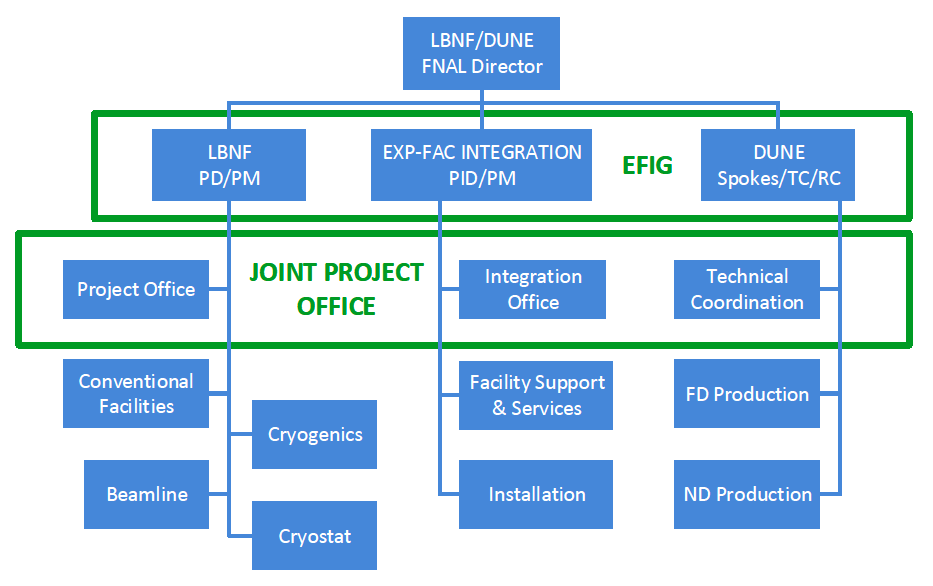
\includegraphics[width=0.99\textwidth]{fs-integration-org-chart} %DUNE_global}
\end{dunefigure}

In addition to the \dword{lbnf} and \dword{dune} elements, the 
overall coordination for integration and installation  
in the excavated, underground caverns is managed as a separate
element of \dword{lbnf-dune} under the responsibility of 
the \dword{ipd}, who is appointed by and reports directly to the 
\dword{fnal} director.  To ensure the best possible coordination 
across \dword{lbnf-dune}, the \dword{ipd} connects 
to facilities through 
ex officio positions on the \dword{lbnf} project management board 
and to detector construction projects through similar positions on the \dword{dune} \dword{exb}.

The \dword{efig} is responsible for the high-level
coordination required between the \dword{lbnf} and \dword{dune} construction 
projects as well as for the integration and 
installation of the \dword{lbnf-dune} pieces. This group, chaired by the \dword{lbnf} project director and \dword{ipd},  operates via  
consensus among its leadership team. 

The \dword{efig} is augmented by a \dword{jpo} that supports the
\dword{lbnf} and \dword{dune} projects as well as integration
across \dword{lbnf} and \dword{dune}. The \dword{jpo} 
combines project activities and functions that exist within the 
\dword{lbnf} and \dword{dune} projects so they  
 coordinate properly across the entire enterprise.    
For a coherent review process across the 
\dword{lbnf-dune} enterprise, reviews will be coordinated 
through the \dword{jpo}. 
Figure~\ref{fig:DUNE_jpo} shows the current organizational 
structure of the \dword{jpo}, indicating the members being 
pulled in from the \dword{lbnf}, \dword{dune} (\dword{tc}), and 
\dword{lbnf}/\dword{dune} integration and installation (Neutrino Platform at \dword{cern}) 
project teams.

\begin{dunefigure}[JPO organization chart]{fig:DUNE_jpo}
  {\dword{jpo} organization chart.}
  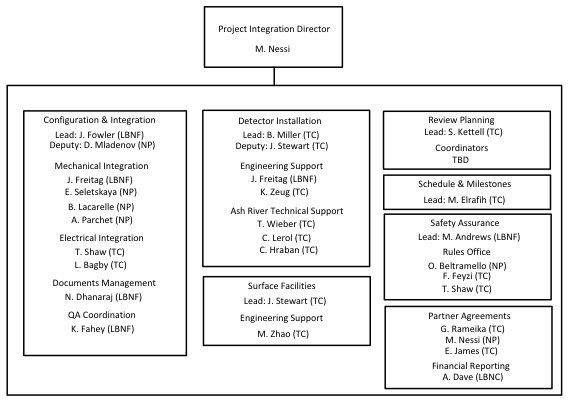
\includegraphics[width=0.99\textwidth]{DUNE_jpo}
\end{dunefigure}


\subsection{Safety}
\label{sec:dune_safety}

\fixme{discuss with Eric on Thursday. Tim says: who's in charge?  We need to look at Steve's volume to reconcile. Anne 7/24}

For a consistent approach to safety across \dword{lbnf-dune},
a single project \dword{esh} manager reports directly 
to the \dword{lbnf} project director, \dword{ipd}, and \dword{dune}
management (via the \dword{dune} \dword{tcoord}).  This manager
directs separate safety teams responsible for implementing the 
\dword{lbnf-dune} \dword{esh} program for both the \dword{lbnf} 
and \dword{dune} projects as well as the \dword{lbnf}/\dword{dune}
integration and installation activities at \dword{surf}.  The 
project \dword{esh} manager works directly with the \dword{fnal} 
and \dword{surf} safety teams to ensure that all project-related 
activities comply with the rules and regulations of the host 
organizations.  The project \dword{esh} manager works with a \dword{jpo} 
engineering safety assurance team to develop
equivalencies in codes and standards across the international project
as needed.

Safety issues related to the handling 
and installation of components are addressed  
from the earliest design reviews through the development 
of detailed engineering notes containing the required
structural analysis.


\subsection{Engineering Integration}
\label{sec:dune_engineering}

\fixme{Let's make sure it sounds like there is one engineering team. Anne}

A central \dword{jpo} engineering team will build 
an integrated model of the detectors within their supporting
infrastructure and the \dword{cf} that house them.  
The \dword{lbnf-dune} project has adopted 
the formal change control process developed previously for the 
\dword{lbnf} project.  The change control process applies to 
proposed changes to requirements, technical designs, 
schedule, overall project scope, and assigned responsibilities 
for individual scope items. 
The \dword{jpo} team incorporates approved design changes as they 
are received and runs a series of checks to ensure that no errors 
or spatial conflicts are introduced into the model. After receiving the 
appropriate sign-offs from all parties, 
The \dword{jpo} team will maintain  
each release  of the model and make it available to the 
design teams as the current release against which the next set 
of design changes is to be generated. 

Electrical engineers are also incorporated within the central
\dword{jpo} team to properly integrate and install 
the detector electrical components.  

The \dword{jpo} engineering team documents and
controls the interfaces between the \dword{lbnf} and \dword{dune} 
projects as well as the interfaces between these projects and the 
\dword{lbnf}/\dword{dune} integration and installation activities 
at \dword{surf}.  


\subsection{Schedule and Milestones}
\label{sec:dune_schedule}

The \dword{jpo} team also creates a single 
project schedule for \dword{lbnf-dune}, incorporating all 
\dword{lbnf} and \dword{dune} activities with the 
integration and installation activities at \dword{surf} 
as well as all interdependencies.  This schedule will 
be used to track the status of the global enterprise.  
  The non-\dword{doe} activities 
will not be tracked using the formal \dword{evms} procedures 
required for the \dword{doe} project activities but rather 
through management teams responsible for those activities who regularly assess progress toward completion.  


\subsection{Partner Agreements and Financial Reporting}
\label{sec:dune_agreements}

Partner contributions to all project elements will be detailed 
in a series of written agreements.  \dword{dune} will create a single \dword{mou} 
detailing the contributions of all participating partners.  
 The  \dword{jpo} will coordinate a series of technical agreements, describing the exact 
boundaries between partner contributions and the terms and 
conditions under which contributions will be delivered. These will accompany
 the primary agreements.   

%%%%%%%%%%%%%%%%%%%%%%%%%%%%%%%%%%%%%%%%%%%%%
\section{Detector Design and Construction Organization}
\label{sec:es-tc-det-const}

The \dword{dune} \dword{fd} construction project refers collectively 
to the activities associated with designing and constructing the
necessary detector components.  \dword{dune} collaboration management 
will oversee this portion of \dword{lbnf-dune} and 
ensure its successful execution.  The high-level \dword{dune} 
collaboration management team, consisting of the co-spokespersons, 
\dword{tcoord}, and \dword{rcoord}, is responsible for day-to-day 
administration of the project.  

Consortia of collaboration institutions, who assume responsibility 
for detector subsystems, construct the \dword{dune} \dwords{detmodule}. Each consortium plans and executes 
construction, installation, and commissioning of its subsystem.  In most cases, a single consortium is responsible for subsystem deliverables supported by 
multiple funding agencies, with each agency managing its own internal projects. 

Each consortium has an overall consortium leader 
and a technical lead.  The consortium leader chairs an institutional 
board comprising one representative from each of the collaborating 
institutions that contribute to the activities of the consortium.  Major 
consortium decisions such as technology selections and assignment of 
responsibilities within the institutions are passed through this institutional 
board.  These decisions are then passed as recommendations to 
the \dword{dune} \dword{exb} for formal collaboration approval.

Because the consortia operate as self-managed entities, a strong
\dword{tc} organization must ensure overall integration 
of the detector elements and successful execution of the detector
construction project.  \dword{tc} areas of responsibility include 
general project oversight, systems engineering, \dword{qa}, and 
safety.  \dword{tc} also supports the planning and execution 
of integration and installation activities at \dword{surf}.  

The \dword{tcoord} manages the overall detector construction project
through regular board meetings with the consortium leadership teams 
and members of the \dword{tc} organization.  
%These board meetings are used to identify and resolve technical issues
%and serve as the primary forums for required interactions between the 
%consortia. Any decisions generated through these board meetings are passed to 
%the \dword{dune} \dword{exb} as recommendations for formal approval.
%
In addition, the \dword{tcoord} heads %an organization 
a project coordination team that supports the work of 
the consortia and has responsibility for a number of major project 
support functions: 
\begin{itemize}
\item ensuring that each consortium has a well defined and complete
  scope, that interactions between consortia are sufficiently 
  well defined, and that any required scope outside the 
  consortia scope is provided through other sources such as collaboration
  common funds;
\item defining and documenting scope boundaries and technical 
  interfaces both between consortia and with \dword{lbnf};  
\item developing an overall schedule with appropriate dependencies
  between activities covering all phases of the project;  
\item ensuring that appropriate engineering and safety standards 
  are developed, understood, and agreed to by all key stakeholders 
  and that these standards are conveyed to and understood by each
  consortium;
\item ensuring that all \dword{dune} requirements on \dword{lbnf} 
  for \dword{cf}, cryostat, and cryogenics are clearly defined and 
  agreed to by each consortium;
\item ensuring that each consortium has well developed and properly reviewed
  component designs, construction plans, \dword{qc} processes, and 
  safety programs; and
\item monitoring the overall project schedule and the progress of 
  each consortium toward delivering its assigned scope. 
\end{itemize}

The \dword{dune} \dword{tc} organizational structure is shown 
in Figure~\ref{fig:DUNE_tc}.  

\begin{dunefigure}[DUNE technical coordination org chart]{fig:DUNE_tc}
  {\dword{dune} \dword{tc} organizational chart.}
  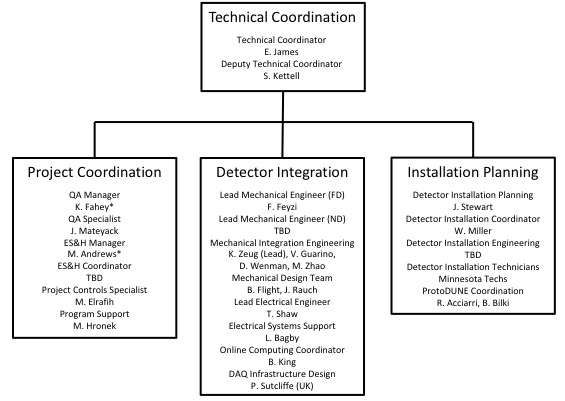
\includegraphics[width=0.99\textwidth]{DUNE_tc}
\end{dunefigure}
\fixme{figure \ref{fig:DUNE_tc} needs replacement per Tim. 7/24 Who has the latest?}

This project coordination team incorporates \dword{esh}, 
\dword{qa}, and project controls specialists.  Engineering support 
is provided through the \dword{tc} detector integration team 
headed by the lead \dword{dune} mechanical and electrical engineers.
Planning coordinators for integration and installation activities 
at \dword{surf} are embedded within both the \dword{jpo} and the 
\dword{tc} installation planning team.  Placing 
these individuals within both organizations facilitates required 
coordination of integration and installation planning 
between the core team directing these activities and the 
\dword{dune} consortia. %, which maintain primary responsibility for the individual detector subsystems.  Members of the \dword{tc} organization meet weekly to review project progress and discuss technical issues. 

The \dword{dune} project has already completed an initial round of design 
and prototyping culminating in the construction and operation 
of the \dword{protodune} detectors.  Moving forward, the project is 
updating detector component designs to incorporate lessons learned from 
the \dword{protodune} experience.  Then the designs are final, the 
project will first construct production versions of all components to be installed and operated in a second phase of \dword{protodune} 
operations before starting full-scale production.  The operation 
of each \dword{protodune2} detector will begin roughly two years after
the end of operations for its corresponding \dword{protodune} detector.
In a few cases, production of components requiring a long lead time must 
be started in parallel with the operation of first production components 
in \dword{protodune2}.

%%%%%%%%%%%%%%%%%%%%%%%%%%%%%%%%%%%%%%%%%%%%%
\section{Integration Engineering}
\label{sec:es-coord-integ-sysengr}

Integration engineering for \dword{dune} focuses on three main functions. The first is configuring the
mechanical and electrical systems of each \dword{detmodule} and managing
the interfaces between them.  The second 
is assuring that the \dwords{detmodule} can be integrated and
installed into their final configuration, and the third is
integrating the necessary services provided by \dword{cf} 
with the \dwords{detmodule}. 

To coordinate these functions, the consortia provide engineering data from their
subsystems to the \dword{tc} engineering team, which maintains subsystem
component documentation.  
These groups create and share
drawings, models, schematics, production data, and all other
engineering documents. In addition, the \dword{tc} engineering team
generates and shares all interface drawings and documentation.
 
\subsection{Mechanical Modeling and Interfaces}
\label{sec:es-tc-mech}

Three dimensional (\threed) mechanical modeling techniques can represent the \dwords{detmodule} well and manage their configurations, but because  \threed modelling techniques vary, a set
of clear and unambiguous \twod integration drawings must first be generated to serve as
the basis for the \threed model accuracy and for the engineering
design of all components. The \twod integration drawings must show the 
interfaces to the level of detail necessary to ensure proper fit and function.  These \threed and 
\twod models are considered static because they do not represent effects of gravity, tolerances, cold
temperature, and installation and assembly clearances.

For installation and operation, however, envelope models  are developed to 
show the effects on the detector 
caused by, among others, distortion of the cryostat and \dword{dss} due to gravity, loads  during 
detector filling and operation, thermal contraction,  as well as tolerances and clearances for tooling.

Interfaces among components are developed, managed, and controlled through additional models and drawings. 
Integration drawings are derived directly from the overall
integration model, which in turn is assembled from
component models developed by the consortia.
\dword{tc} is responsible for controlling many of these interfaces. 

\subsection{Electrical Designs and Interfaces}
\label{sec:es-tc-elec}

\dword{tc} is responsible for the \dword{ac} power
distribution supplied to the experiment and to detector electronics
racks.  Through the design review process, \dword{tc} will  ensure 
that all electrical systems  follow safe design practices and
will pass \dwords{orr}. We will follow the same  guidelines\cite{bib:cernedms2095958} for \dword{dc} power supplies as
were followed at \dword{protodune} and developed during extensive testing of
the \dword{apa} wire readout at \dword{bnl} for \dword{protodune}.  

The electrical design of each subsystem is described by a set of
documents that includes a system-level block diagram and a wiring
diagram with a complete description of all power and ground
connections. Interfaces that occur between subsystems of different consortia must be documented and formally agreed upon between the technical leads of the coordinating 
consortia and must be verified by the \dword{tcoord} team.  All systems are reviewed for compliance to the guidelines during the design review procedure, and deviations  are noted and approved by system engineering. 

The \dword{tc} team will provide unique names and labels
for all racks, crates, boards, power supplies, cables, and any other
electrical type equipment.  A database will be created to track these
devices.

\subsection{Integration}
\label{sec:es-tc-integ}

 An integration mechanism has been developed to manage and create an overall model of interfaces both within a \dword{detmodule} and between a \dword{detmodule} and facilities.
 The \dword{jpo} engineering team carries out  and manages interfaces between the nodes.

\begin{dunefigure}[Integration Nodes]{fig:integration_nodes}
  {Overall integration nodes and interfaces.}
  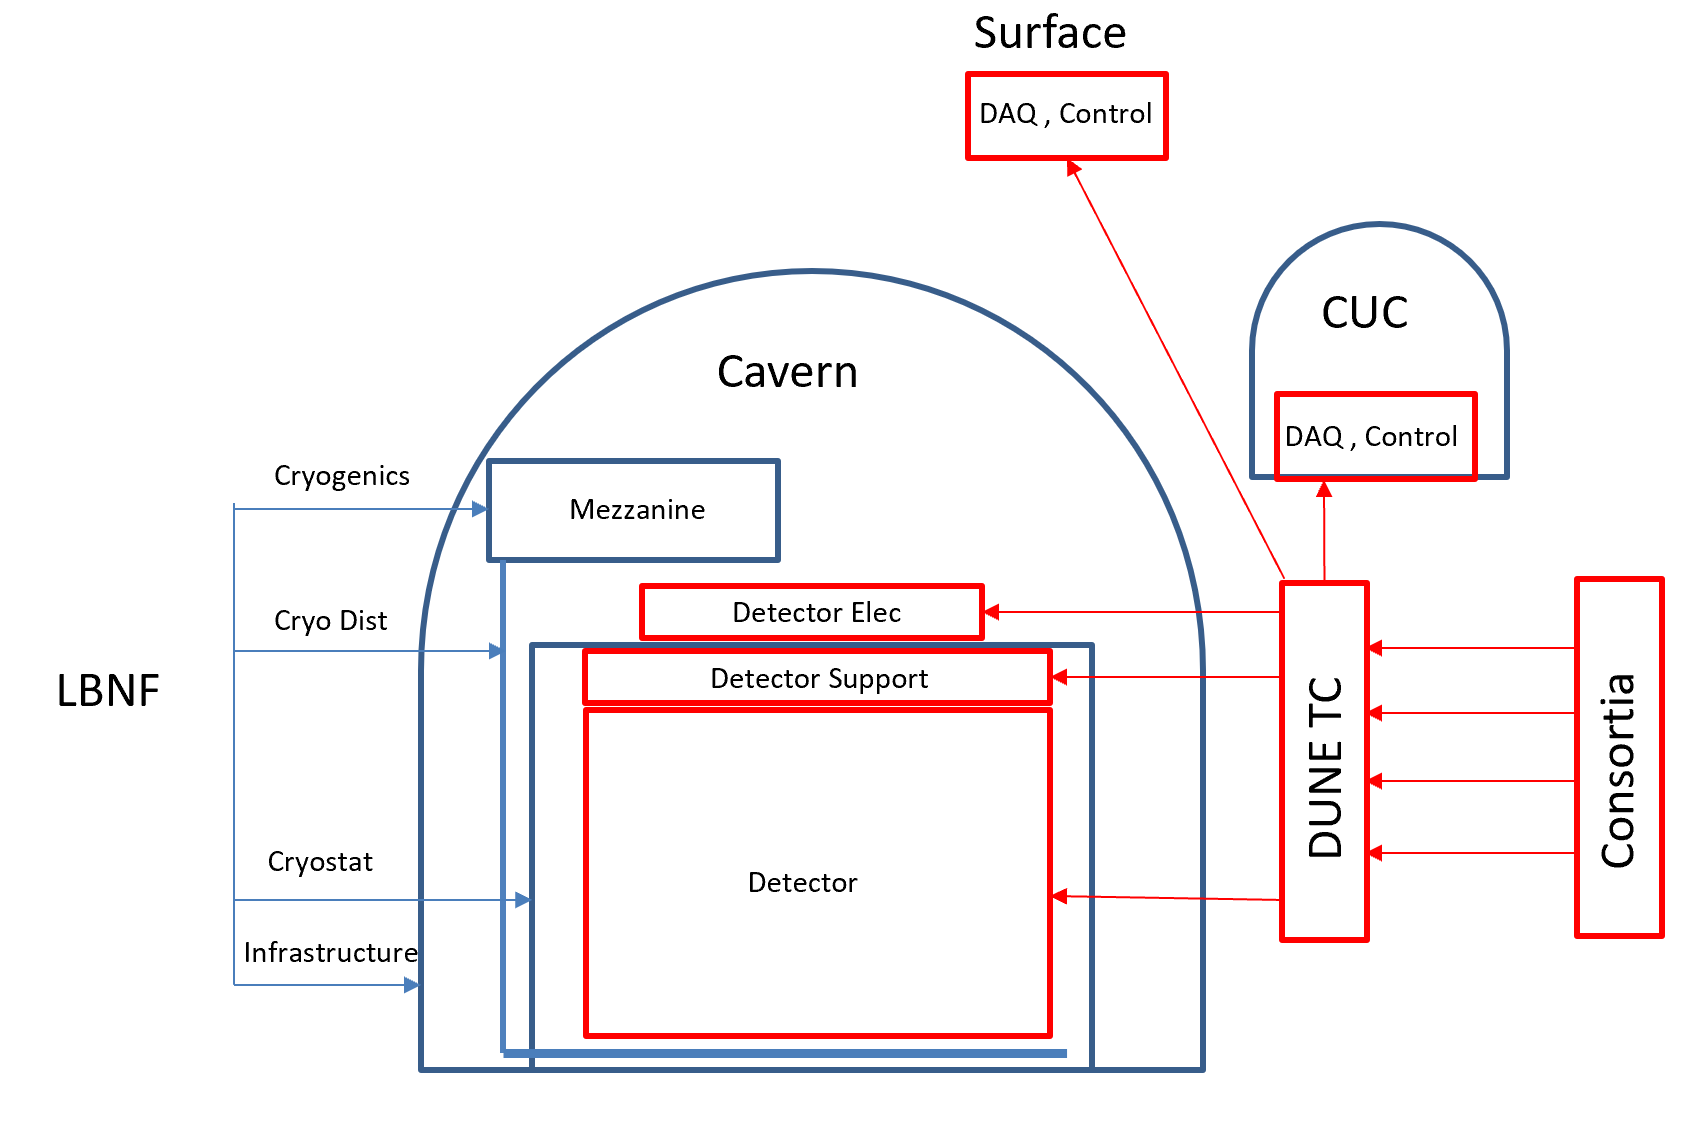
\includegraphics[width=0.7\textwidth]{Integration_nodes.png}
\end{dunefigure}

Figure~\ref{fig:integration_nodes} shows the interfaces between the
detector and facilities. In this figure, within the cavern, items
provided by \dword{lbnf} are on the left and the items provided by
\dword{dune} are on the right. In addition, the \dword{tc} engineering
team ensures connectivity between the \dword{daq} room in the \dword{cuc} and
surface control and network rooms. \fixme{prev sentence unclear - what does it mean to integrate these rooms? anne} Interface documents are developed and maintained to manage the
interfaces %among 
between consortia and between %consortia 
each consortium and the  \dword{tcoord}. At the time of this writing, not all
documents have been fully developed. Once the technical design is
finished, the interface documents will be placed under revision
control.

\subsection{Value Engineering}
\label{sec:es-tc-fdsp-coord-ve}

Value engineering is the process of arriving at cost-effective
solutions to the technical challenges of building the \dword{dune}
detector. \dword{dune} value engineering builds on significant
developments in \dword{lar} detectors dating to the early 1970s,
especially the large \dwords{lartpc} \dword{icarus} and
\dword{microboone}. Prototypes up to and including the \dword{protodune} 
detectors have been used to validate
\dword{dune} designs and confirm the necessary performance. 

Value engineering is ongoing at all stages of design and will continue
through fabrication, assembly, and installation phases. In
particular, during the fabrication and assembly stages, when labor costs
are relatively higher, this can result in significant cost savings. 

%%%%%%%%%%%%%%%%%%%%%%%%%%%%%%%%%%%%%%%%%%%%%
\section{Reviews}
\label{sec:es-tc-reviews}


The \dword{jpo} and \dword{tc} review all stages of detector development
and work with each consortium to arrange reviews of the design
(\dword{cdrev}; \dword{pdr} and \dword{fdr}); production (\dword{prr}
and \dword{ppr}); installation (\dword{irr}); and operation
(\dword{orr}) of their system.  These reviews provide information to
the \dword{tb} and \dword{exb} to help them evaluate technical
decisions. A timeline for the review process is shown in
Figure~\ref{fig:review_timeline}.
\begin{dunefigure}[DUNE review process]{fig:review_timeline}
  {\dword{dune} review process and timeline.}
  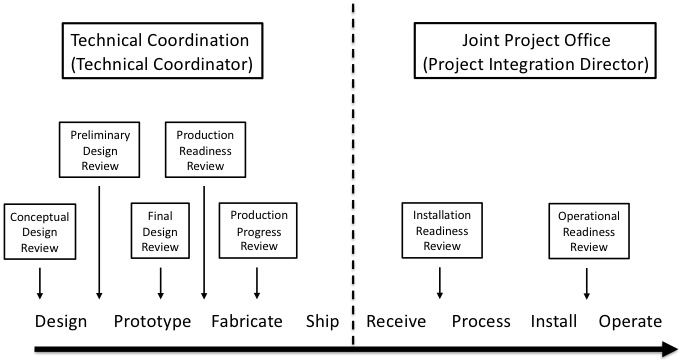
\includegraphics[width=0.75\textwidth]{review_timeline}
\end{dunefigure}

Production of detector elements begins only after successful
\dwords{prr}. Regular production progress reviews will be held once
production starts. 

The review process is an important part of the \dword{dune} \dword{qa}
process for design and production.

%%%%%%%%%%%%%%%%%%%%%%%%%%%%%%%%%%%%%%%%%%%%%
\section{Quality Assurance}
\label{sec:es-tc-qa}

The primary objective of the \dword{lbnf-dune} \dword{qa} program is
to assure quality in the construction of the \dword{lbnf} facility and
\dword{dune} experiment while protecting
\dword{lbnf-dune} personnel, the public, and the environment. The
\dword{qa} plan aligns \dword{lbnf-dune} \dword{qa} activities, which
are spread around the world, with the principles of the \fnal Quality
Assurance Manual. The manual identifies the \fnal Integrated Quality
Assurance Program features that serve as the basis for the
\dword{lbnf-dune} \dword{qa} plan.

The \dword{lbnf-dune} \dword{qa} plan incorporates 
a graded approach; it applies a level of analysis,
controls, and documentation commensurate with the potential for any effect on
environment, safety, health, or quality.

One part of the \dword{tc}'s centralized project
coordination functions is
standardizing \dfirst{qa}/\dfirst{qc} practices, one facet
of which is to assist consortia in defining and implementing
\dword{qa}/\dword{qc} plans that maintain uniform high
standards across the entire detector construction
effort. Figure~\ref{fig:fnal_qa} shows how \dword{dune} \dword{tc}
derives its \dword{qa} program from the principles of the \fnal \dword{qa} program:
requirements are flowed down through the \dword{lbnf-dune}
\dword{qa} program into the \dword{qc} plans developed for consortia fabricating detector components and integrating and installing the detector.

\begin{dunefigure}[\fnal QA]{fig:fnal_qa}
  {Flow-down of \fnal \dword{qa} to consortia.}
  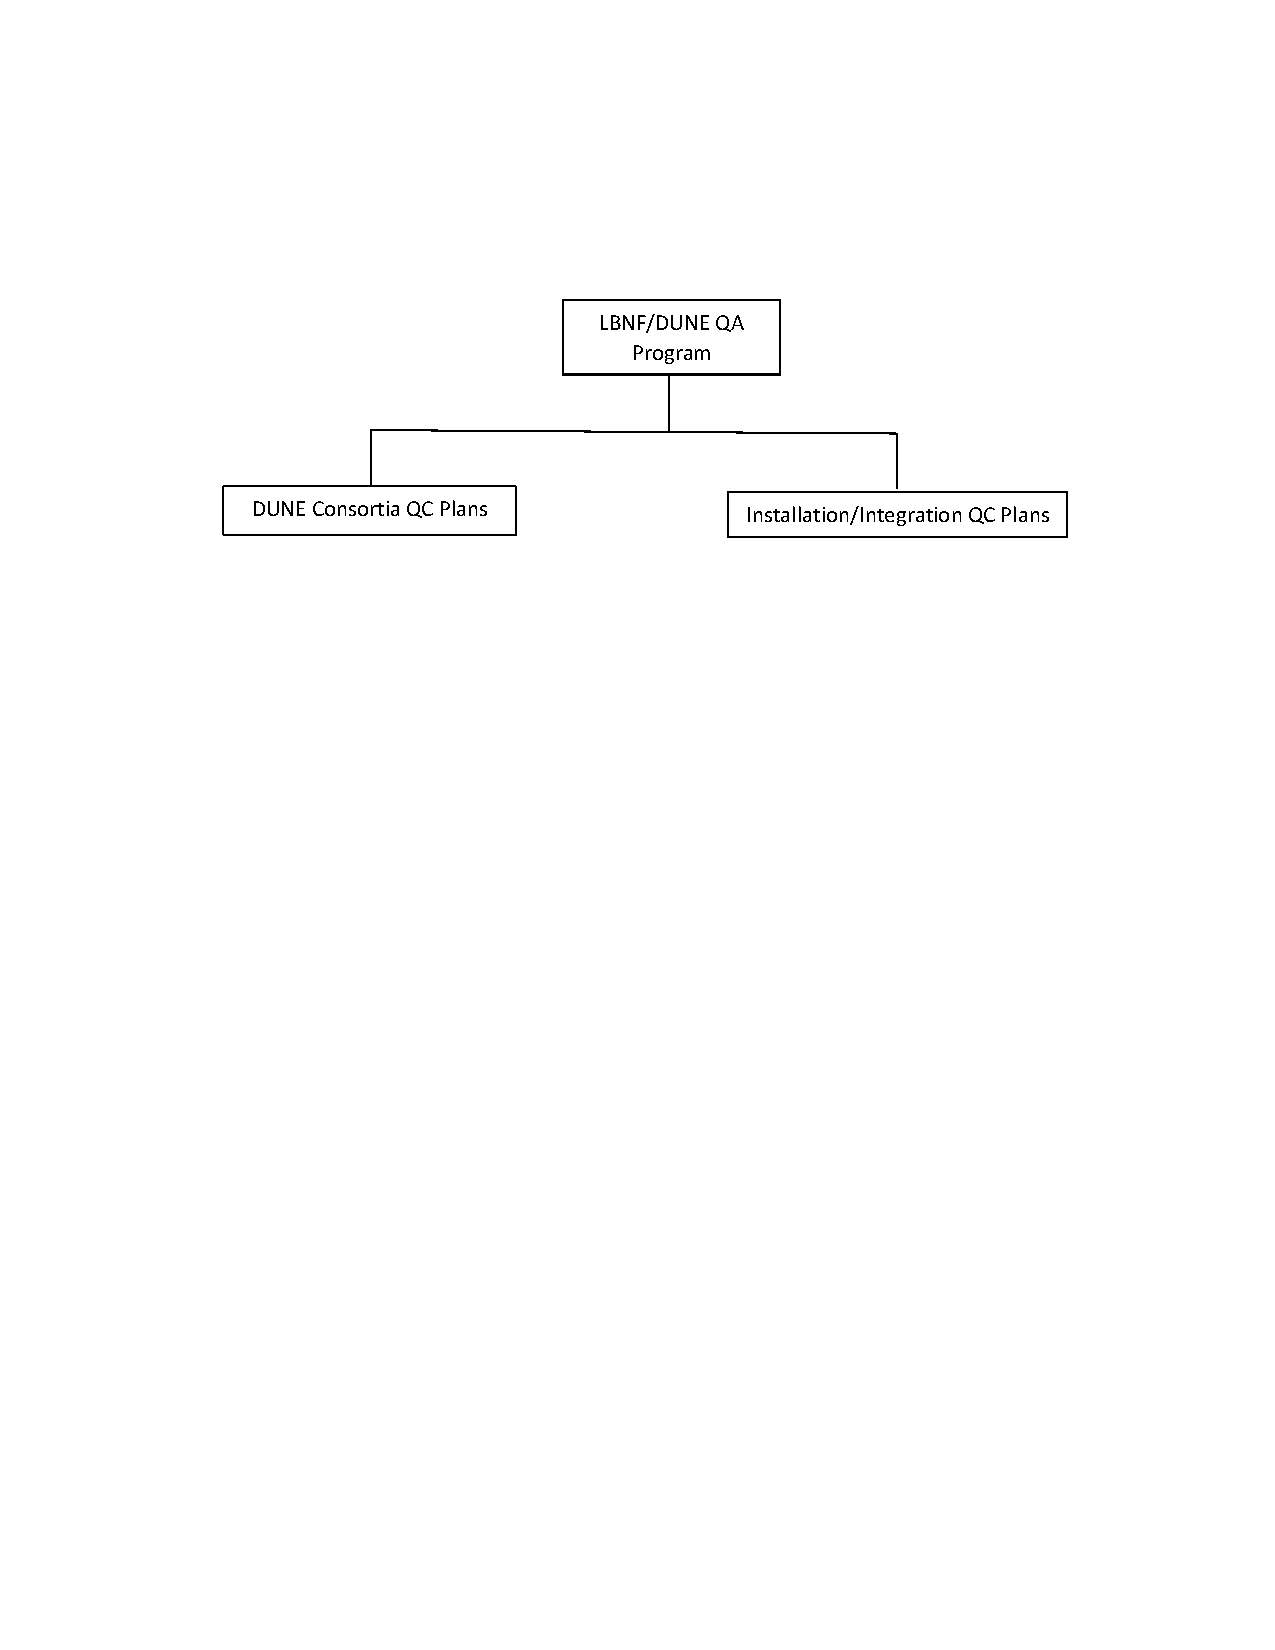
\includegraphics[width=0.85\textwidth]{fnal_qa.pdf}
\end{dunefigure}

The \dword{qa} effort includes design, production readiness and
progress reviews as appropriate for the \dword{dune} detector
subsystems as was done for \dword{pdsp} under \dword{tc}
oversight. Continuous improvement through documentation of lessons learned and best practices is
an integral part of the program. 


The \dword{dune} consortium leaders identify the
resources to ensure that their team members are adequately trained and
qualified to perform their assigned work. 
All consortia members, in turn, are responsible for the quality of the work that
they do and for using available guidance and assistance. All members 
have the authority to stop work and report adverse conditions that
affect the quality of \dword{dune} products to their 
\dword{dune} consortium leader and the \dword{lbnf-dune}
\dword{qa} manager. The \dword{qa} plan
defines the \dword{qa} roles and responsibilities within the \dword{dune}
project.


%%%%%%%%%%%%%%%%%%%%%%%%%%%%%%%%%%%%%%%%%%%%%
\section{Environment, Safety, and Health}
\label{sec:es-tc-eshq}

\subsection{The DUNE ES\&H Program}
\label{sec:es-tc-eshq-prog}

\dword{fnal} and \dword{lbnf-dune} are committed to protecting the health and
safety of staff, the community, and the environment, as stated in the
\dword{lbnf-dune} integrated \dword{esh} plan.  The
\dword{esh} program complies with applicable standards as well as local,
state, and federal legal requirements through the \dword{fnal} Work Smart set
of standards and the contract between \dword{fra} and the
\dword{doe} Office of Science (\dword{fra}-\dword{doe}). \dword{fnal}, as the host
laboratory, established the \dword{sdsd} to provide
facility support.  The \dword{sdsd} is responsible
for \dword{lbnf-dune} operations at \dword{surf}.

The \dword{lbnf-dune} \dword{esh} management system is
designed to work hand-in-hand with the \dword{surf} emergency
management systems to protect workers, the public, and the environment.
 Doing so helps in executing the
scientific mission.  \dword{fnal} uses a set of criteria to plan, direct,
control, coordinate, assure, and improve how \dword{esh} policies,
objectives, processes, and procedures are established, implemented,
monitored, and achieved. \fixme{that's quite  a sentence! Also - these criteria must be from the work smart standards?}



The \dword{tcoord} and \dword{ipd} are responsible for
implementing the \dword{dune} \dword{esh} program.  The
\dword{lbnf-dune} \dword{esh} manager reports directly to the
\dword{tcoord} and \dword{ipd} and provides
\dword{esh} support and oversight for developing and implementing the
\dword{lbnf-dune} \dword{esh} program. The \dword{dune} \dword{esh}
coordinator reports to the \dword{lbnf-dune} \dword{esh}
manager and has primary responsibility for \dword{esh} support and
oversight of the \dword{dune} \dword{esh} program for all activities
at collaborating institutions and at \dword{lbnf-dune}
facilities located at \dword{surf}. The \dword{lbnf-dune} \dword{esh} plan defines the \dword{esh}
requirements applicable to installation activities at \dword{surf}. 

The \fnal \dword{esh} Section, \dword{doe}, and
\dword{lbnf} \dword{esh} have completed a series of assessments of
critical \dword{sdsta} \dword{esh} programs including underground access,
emergency management, electrical safety, rigging, and fire
protection. It tracks the findings and lessons learned identified in these
 and other reviews and assessments, 
disseminate them where applicable, and ensure they are appropriately implemented.

\subsection{Hazard Identification}
\label{sec:es-tc-eshq-har}

A key element of an effective \dword{esh} program is identifying hazards. 
Once a list of hazards has been compiled for a facility, these hazards can be screened
and managed through a suitable set of controls.

The \dword{lbnf-dune} project completed a Hazard Analysis Report (\dword{har})
to ensure that identified hazards are mitigated early in the
design process.  The focus of the report is process hazards,
not activity hazards, which are typically covered in a job hazard
analysis.  The \dword{har}  identifies
hazards anticipated in the project's construction and operational
phases, proposes ways to mitigate the hazards to reduce risk, and establishes a
post-mitigation risk category for each.  As the \dword{dune} design 
matures, the \dword{har} will be
updated to ensure that all hazards are properly identified and
controlled through design and safety management programs.

\subsection{Codes/Standards Equivalencies}
\label{sec:es-tc-esh_codes}

\dword{dune} will rely on significant contributions from international
partners. In many cases, an international partner will contribute
equipment to be installed at \dword{surf} or \dword{fnal} 
that was built following one of the
international standards or directives. \dword{fnal} has established a
process, detailed in \dword{feshm} Chapter 2110, to establish code
equivalency between US and international engineering design codes
and standards. This process allows the laboratory to accept in-kind
contributions from international partners or purchase equipment
designed using international standards while ensuring a level of safety equivalent or
higher than US engineering codes and standards.


\subsection{ES\&H Requirements at Collaborating Laboratories and Institutions}

All \dword{dune}-related work performed at collaborating institutions will be completed
following the collaborating institution's \dword{esh} policies and
programs. Equipment and operating procedures provided by the
collaborating institution will conform to the \dword{dune} project
\dword{esh} and integrated safety management policies and
procedures. The \dword{esh} organization at collaborating institutions
must provide \dword{esh} oversight for all work activities carried
out at their institution facilities. \dword{lbnf-dune}
personnel will also follow the \dword{esh} manual and procedures while at
the collaborating institutions.

\subsection{LBNF-DUNE ES\&H Program Requirements at SURF}

Special site and facility access requirements are in place for the \dword{surf} site. All \dword{dune} workers requiring access to the \dword{surf} site must
register through the \fnal Users Office and apply for
a \dword{surf} identification badge as part of
the \dword{surf} Site Access Control Program.
This program also requires a \dword{tap} for each daily access to the
underground areas.  All personnel within each working group must be
individually listed on the \dword{tap} and must brass in and
out using the brass board at the entrance to the Ross Shaft
cage before and after accessing the underground facilities. Personnel shall wear the required \dword{ppe} when on site at \dword{surf}. 
A detailed list of the \dword{ppe} appears in \tcchesh. 


Each \dword{dune} collaborator, as part of registration through the \fnal Users office,
will complete the user \dword{esh} training modules, and the supervisor
will complete a training needs assessment to develop a training plan
to define additional \dword{dune} \dword{esh} training requirements for the collaborator.
In addition, all personnel performing work on-site at \dword{surf} must
attend \dword{surf} \dword{esh} Site Orientation before beginning work at the site.


%A work planning and hazard analysis process is in place to initiate thought about the hazards associated with work and how it can be performed safely.  
All work activities
shall be subject to work planning and hazard analysis. 
Work planning ensures the scope of
the job is understood, appropriate materials are available, all
hazards have been identified, mitigation efforts established, and all
affected employees understand what is expected of them.   
All work planning documentation will be reviewed and
approved by the \dword{dune} \dword{esh} coordinator and the \dword{dune}
\dword{esh} review committee before beginning work activities.

A safety data sheet must be supplied for all chemicals and
hazardous materials used on site. All chemicals and hazardous
materials brought to the \dword{surf} site must be reviewed/approved by the
\dword{dune} \dword{esh} coordinator and the \dword{surf} \dword{esh}
department before arriving on site.

An emergency management program will be in place that incorporates an \dword{ert},  trained guides on all underground levels during all shifts, and protocols for treating injuries, accidents, or spills.

Fire and life safety requirements for \dword{lbnf-dune} areas
were analyzed in the \dword{lbnf-dune} Far Site Fire and Life
Safety Assessment. All caverns will be equipped with fire detection
and suppression systems with both visual and auditory notification.  
\dword{surf} will monitor all fire alarms and system supervisory signals, and the \dword{surf} \dword{ert}. 
will respond to the signals, with additional support from the local Lead-Deadwood Fire
Department as needed.  The caverns will also be equipped
with an \dword{odh} monitoring and alarm system with independent visual and
auditory notification systems.


All workers on the \dword{dune} project have the
authority to stop work in any situation that presents an imminent
threat to safety, health, and the environment. Work may not resume
until the circumstances are investigated and deficiencies corrected,
including the concurrence of the \dword{dune} \dword{ipd}
and the \dword{lbnf-dune} \dword{esh} manager.


